% ============================================
% ===== ANEXO 3: FLUJO DE TRABAJO API CANARY =====
% ============================================

\chapter{Flujo de trabajo de la API Canary}
\label{anexo:flujo-canary}

\subsection*{Diagrama}

\begin{figure}[h!]
    \centering
    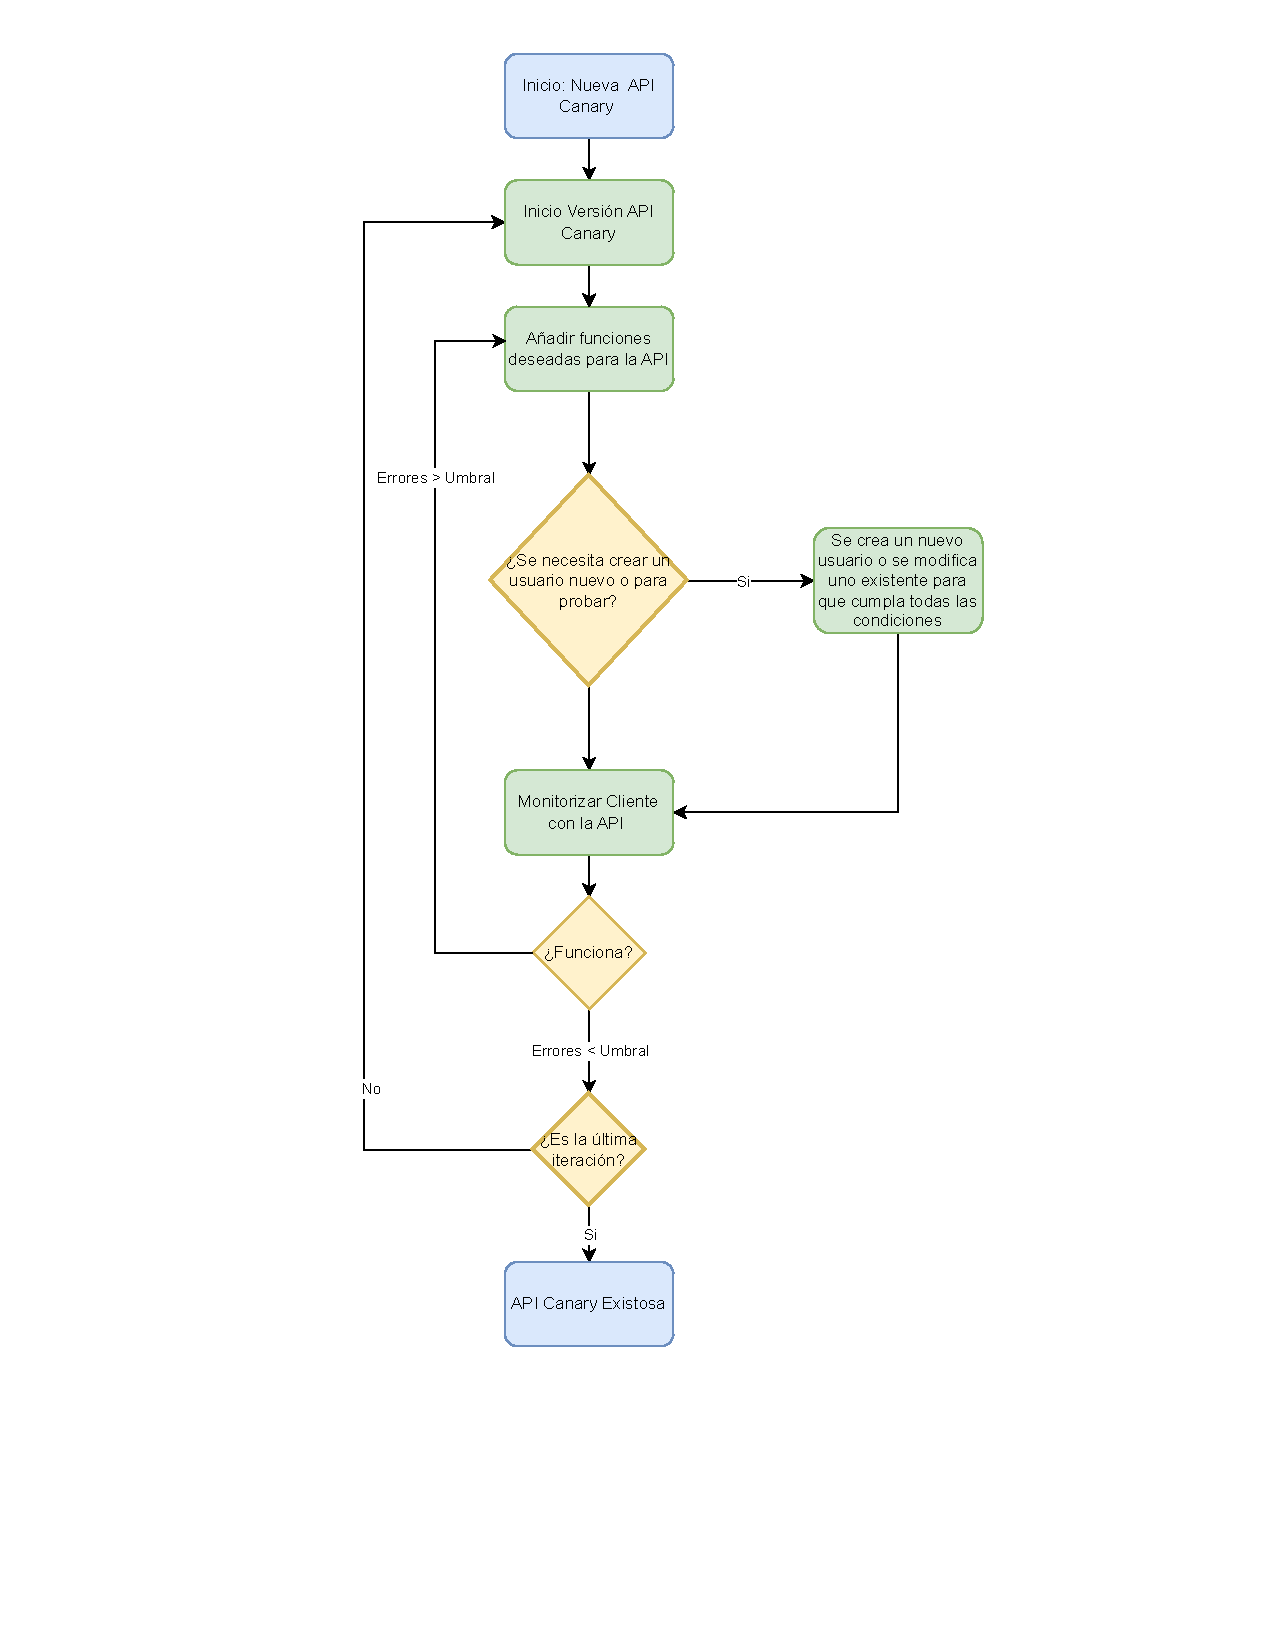
\includegraphics[width=0.9\textwidth]{archivos/flujo_API_Canary.drawio.pdf}
    \caption{Diagrama de flujo del proceso de despliegue Canary para APIs}
    \label{fig:canary-flow}
\end{figure}

\subsection*{Descripción del flujo}

\begin{enumerate}
    \item \textbf{Inicio: Nueva API Canary} --- Desarrollo de una nueva API de validación.

    \item \textbf{Inicio: Nueva versión de la API Canary} --- Inicio de una nueva iteración sobre la API existente, incorporando las funciones planificadas para esa fase.

    \item \textbf{Implementación de nuevas funciones} --- Se añaden las funcionalidades deseadas en el código de la API.

    \item \textbf{Comprobación del usuario de muestra} --- Se verifica que el usuario empleado para las pruebas dispone de todos los recursos necesarios. Si no es así, se ajusta su perfil o se crea uno nuevo que los incluya.

    \item \textbf{Monitorización de métricas} --- Análisis continuo de errores, latencia y otras métricas clave durante la ejecución.

    \item \textbf{Decisión basada en umbrales:}
          \begin{itemize}
              \item \textbf{Errores $<$ umbral} $\rightarrow$ La iteración se considera superada y se avanza a la siguiente fase.
              \item \textbf{Errores $>$ umbral} $\rightarrow$ Se realiza un \textit{rollback} automático a la versión estable anterior y se revisan los cambios para corregirlos.
          \end{itemize}

    \item \textbf{API Canary completada} --- Tras superar todas las fases, la API queda integrada y se programa su ejecución periódica automática.
\end{enumerate}




